

\section{Schwachstelle 11: Schwaches Passwort des Benutzers Lightman auf Host Esperanza}
\label{sec:vuln11}
Aus den vom vorherigen Kapitel extrahierten Passwort-Hashes konnte das Passwort des \texttt{Lightman}-Benutzers mit einem einfachen Wörterbuchangriff aufgedeckt werden. Mit dem Passwort des Lightman-Benutzers sowie den SYSTEM-Rechten aus dem vorherigen Kapitel konnte sich über die RDP-Sitzung auf den Host \texttt{Esperanza} mit dem Benutzer \texttt{Lighman} angemeldet werden.


\subsection{Wegbeschreibung der Schwachstelle}
\label{subsec:vuln11_way}

Um einen Wörterbuchangriff auf die NTLM-Passworthashes fahren zu können, wurden die Hashwerte in der Datei \texttt{ntlm\_hashes\_esperanza.txt} (siehe Textauszug \ref{lst:esperanza_hashwerte}) abgespeichert. 

\lstset{language=bash,caption={Hashwerte vom Host Esperanza}, label=lst:esperanza_hashwerte}
\begin{lstlisting}[frame=single, firstnumber=1, stepnumber=1,]
|--(gu4c4m0l3@kali-t470)-[~/Documents/pentest_MB-Reps/esperanza]
|-$ cat ntlm_hashes_esperanza.txt                                                                 
Administrator:e397497cfbd040ed50c21c92931e2e03
Lightman:2049b70ec5b6944aed5fef05bc4b1933

\end{lstlisting} 


Anschließend konnte das Passwort mit dem Befehl \texttt{sudo hashcat -m 1000 -a 0 --username ntlm\_hashes\_esperanza.txt /usr/share/wordlists/rockyou.txt} innerhalb weniger Sekunden gebrochen werden. Abbildung \ref{fig:vuln10_hashcat_lightman} zeigt dabei die Ausführung des Befehls. Im roten Rahmen wird neben dem Hashwert hinter dem Doppelpunkt das dazugehörige Passwort \texttt{joshua} angezeigt, welches zum Benutzer \texttt{Lightman} zugeordnet werden kann. Das Administrator-Passwort konnte selbst mit weiteren Passwort-Regeln \textbf{nicht} mit einem Wörterbuchangriff gebrochen werden.


\begin{figure}[h]
    \centering
    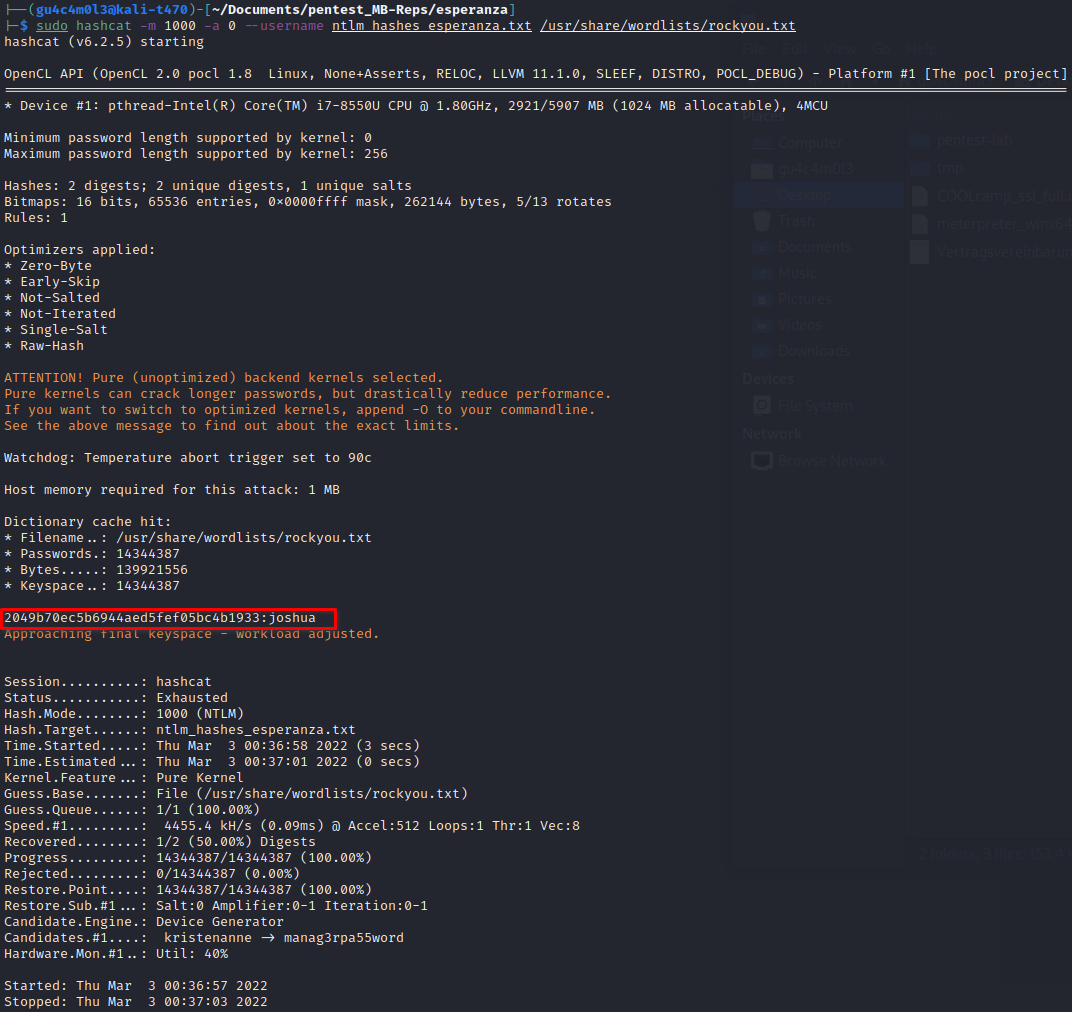
\includegraphics[width=\textwidth]{./img/vuln10_esperanza/hashcat_lightman}
    \caption{Brechen des Passwort-Hashes vom Benutzer \texttt{Lightman} mittels \texttt{hashcat}.}
    \label{fig:vuln10_hashcat_lightman}
\end{figure}

Anschließend wurde versucht über den aus dem vorherigen Kapitel aufgebauten SSH-SOCKS-Proxy-Tunnel sich mittels RDP und dem Benutzernamen \texttt{Lightman} und Passwort \texttt{joshua} am Host \texttt{Esperanza} anzumelden. Da der Benutzer \texttt{Lightman} aufgrund fehlender Gruppen-Berechtigungen keine Anmeldung über RDP erlaubt (s. Fehlermeldung in Abbildung \ref{fig:vuln10_rdp_login_failed}), musste über die Meterpreter-Sitzung mit SYSTEM-Berechtigungen zum \texttt{Esperanza}-Host der Benutzer zur Gruppe \texttt{Remotedesktopbenutzer} mit dem Befehl \texttt{net localgroup "{}Remotedesktopbenutzer"{} "{}Lightman"{} /add} hinzugefügt werden.

\begin{figure}[h]
    \centering
    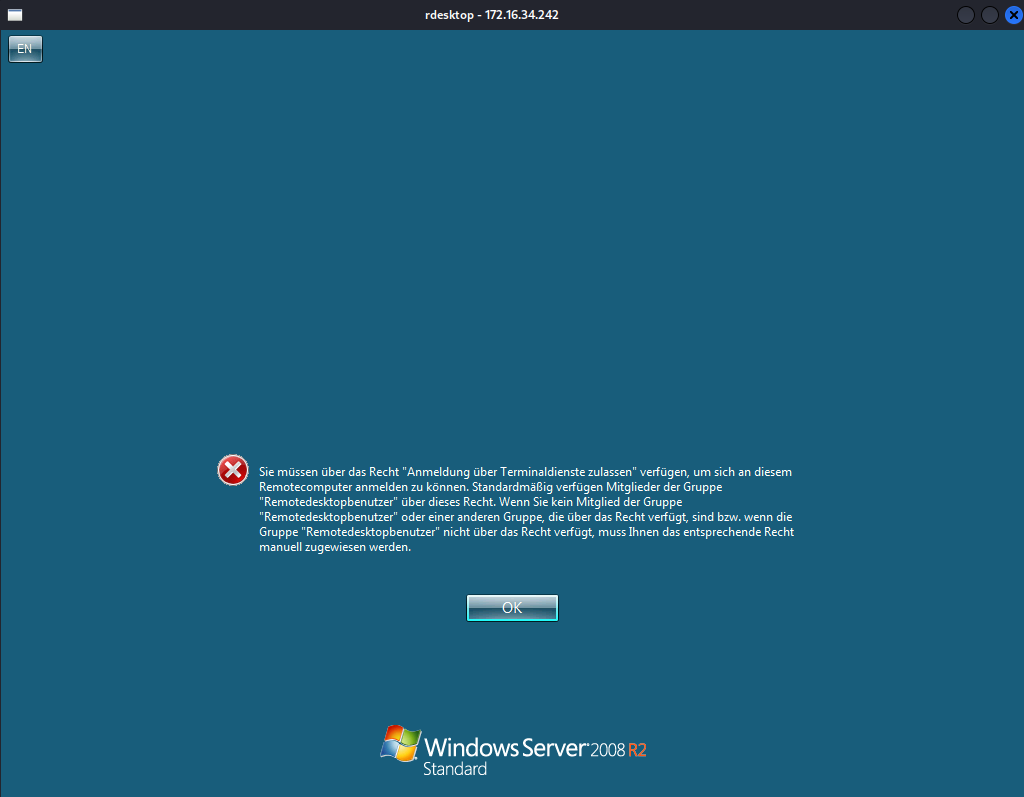
\includegraphics[width=\textwidth]{./img/vuln10_esperanza/rdp_login_not_allowed}
    \caption{RDP-Login aufgrund fehlender Gruppen-Berechtigung für Benutzer \texttt{Lightman} fehlgeschlagen.}
    \label{fig:vuln10_rdp_login_failed}
\end{figure}



Anschließend konnte erneut mit dem Befehl \texttt{proxychains -f proxychains\_bigcindy.conf rdesktop 172.16.34.242} die RDP-Sitzung gestartet und der Benutzer \texttt{Lightman} erfolgreich am System angemeldet werden (siehe Abbildung \ref{fig:vuln10_rdp_login_successful}).

\begin{figure}[h]
    \centering
    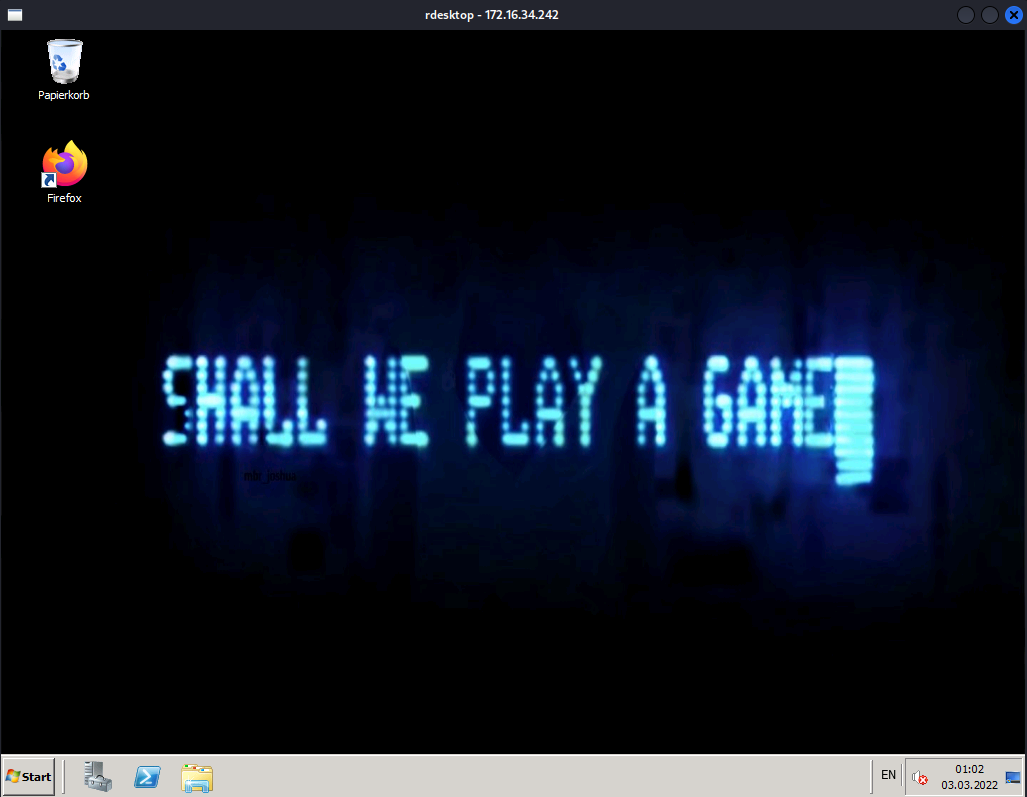
\includegraphics[width=\textwidth]{./img/vuln10_esperanza/rdp_login_ok}
    \caption{Erfolgreicher RDP-Login mit Benutzer \texttt{Lightman} auf \texttt{Esperanza}.}
    \label{fig:vuln10_rdp_login_successful}
\end{figure}





\subsection{Risikobewertung}
TODO

Das Gesamtrisiko wurde daher mit \textcolor{red}{HOCH} bewertet.

\subsection{Empfohlene Gegenmaßnahmen}
TODO

\subsection{Hinterlassene Spuren und Spurenbeseitigung}
Es wurden keine Dateien geändert, hinzugefügt oder Prozesse gestartet.




\lstset{language=bash,caption={TODO}, label=lst:vuln4_TODO}
\begin{lstlisting}[frame=single, firstnumber=1, stepnumber=1,]

\end{lstlisting} 


































